\begin{wrapfigure}[0]{r}[9pt]{0cm}
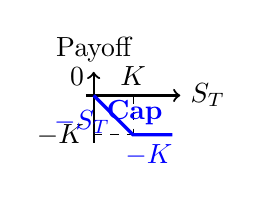
\begin{tikzpicture}[scale=1]
    % --- 定义坐标和参数 ---
    \def\K{0.5}       % 执行价格 K
    \def\maxST{1}     % S_T 的最大显示范围
    \def\minPayoff{-0.5} % Payoff 的最小显示范围 (因为 Cap 的收益为负)

    % --- 绘制坐标轴 ---
    % X 轴 (S_T)
    \draw[->, thick] (-0.1, 0) -- (\maxST + 0.1, 0) node[right] {$S_T$};
    % Y 轴 (Payoff)，向下延伸
    \draw[->, thick] (0, \minPayoff - 0.1) -- (0, 0.3) node[above] {Payoff};

    % --- 绘制辅助线和标签 ---
    % 在 x 轴上标记 K
    \draw[dashed, thin] (\K, 0) node[above] {$K$} -- (\K, -\K);
    % 在 y 轴上标记 -K (Cap 的最大损失水平)
    \draw[dashed, thin] (0, -\K) node[left] {$-K$} -- (\K, -\K);
    % 标记原点
    \node[above left] at (0,0) {0};

    % --- 绘制组成部分 (灰色虚线) ---
    % 1. Short Underlying Asset (Payoff = -S_T)
    % 通过原点，斜率为 -1 的直线
    %\draw[gray, dashed, thick] (-0.1, 0.1) -- (\maxST, -\maxST);


    % 2. Long K-strike Call Option (Payoff = max(S_T - K, 0))
    % 在 S_T < K 时为 0，在 S_T > K 时斜率为 1
   % \draw[gray, dashed, thick] (0, 0) -- (\K, 0) -- (\maxST, \maxST - \K);


    % --- 绘制最终的 Cap Payoff (蓝色粗线) ---
    % Cap Payoff = Long Call + Short Asset = max(S_T - K, 0) - S_T
    % 当 S_T <= K 时，Payoff = 0 - S_T = -S_T
    % 当 S_T > K 时，Payoff = (S_T - K) - S_T = -K
    \draw[blue, very thick] (0, 0) -- (\K, -\K) -- (\maxST, -\K);

    % --- 添加简化的标签 ---
    % 斜线段的 Payoff = -S_T
    \node[blue, left] at (\K/1.5, -\K/1.5) {$-S_T$};
    % 水平段的 Payoff = -K
    \node[blue, below] at (\K + 0.2, -\K) {$-K$};
    % 总标签
    \node[blue, anchor=south east] at (\maxST, -\K) {\textbf{Cap}};

\end{tikzpicture}
\end{wrapfigure}